\section{Robottens højde}
\label{DatabehandlingRHeight}
%
I dette afsnit analyseres resultaterne med udgangspunkt i de fem forskellige højder robotten havde i testen. For hver højde er der mellem 7-10 testpersoner. De forskellige højder fremgår af \autoref{tab:RHeight}, hvor antallet af testpersoner ligeledes er opgivet. Det undersøges, hvordan robottens højde påvirker de rejsendes oplevelse af robotten ved at undersøge, hvordan resultaterne ændrer sig afhængigt af de fem forskellige højder. Det er et \textit{Between-subject} design, da hver testperson kun har oplevet robotten i én af højderne og svaret ud fra denne.
%
\begin{table}[H]
\centering
\begin{tabular}{c|c}
Højde (cm) & Antal testpersoner \\ \hline
118   & 9     \\ \hline
123.5 & 10    \\ \hline
129   & 9     \\ \hline
140   & 7     \\ \hline
151   & 8      \\
\end{tabular}
\caption{Oversigt over antallet af testpersoner til hver af de fem højde robotten havde.}
\label{tab:RHeight}
\end{table}
\noindent
%
Ud fra \textit{Scree}-plottet på \autoref{fig:RHeight-Scree} fremgår det, at cirka 80 \& af variansen kan forklares ud fra de to første \textit{Principal Components} (PCs). Ved at tage PC3 med opnås cirka 94 \% forklaret varians. Det er dog væsentligt simplere at fortolke resultaterne i to dimensioner og der fokuseres derfor som udgangspunkt kun på de to primære komponenter.
%
\begin{figure}[H]
\centering
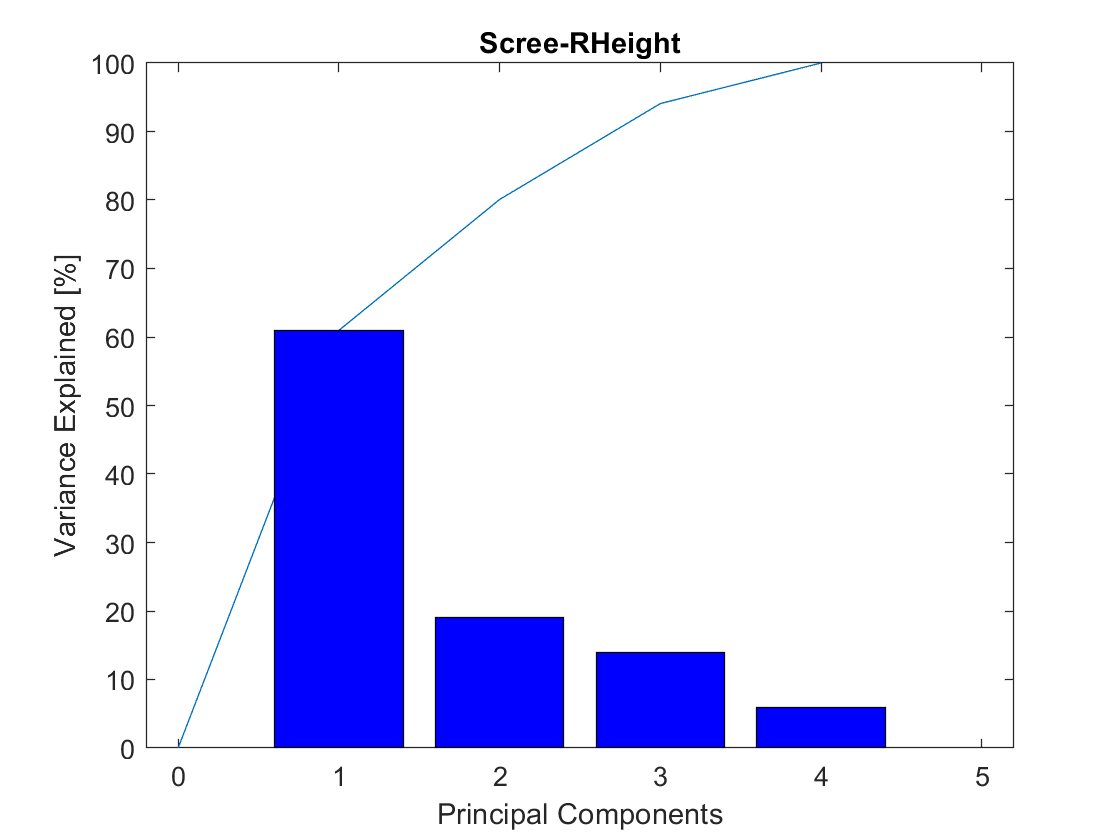
\includegraphics[width=\textwidth]{Figure/DatabehandlingSkalaer/PCAfigures/RHeight-Scree.png}
\caption{\textit{Scree}-plot, hvorpå sammenhængen mellem antallet af \textit{Principal Components} og \textit{Variance Explained [\%]} fremgår.}
\label{fig:RHeight-Scree}
\end{figure}
\noindent
%
Ud fra \textit{Score}-plottet på \autoref{fig:RHeight-Score} fremgår det, at der generelt er en del spredning mellem resultaterne ud fra de fem forskellige højder, men at 129 cm og 140 cm har lignende karakteristikas, da de ligger meget tæt i plottet.
%
\begin{figure}[H]
\centering
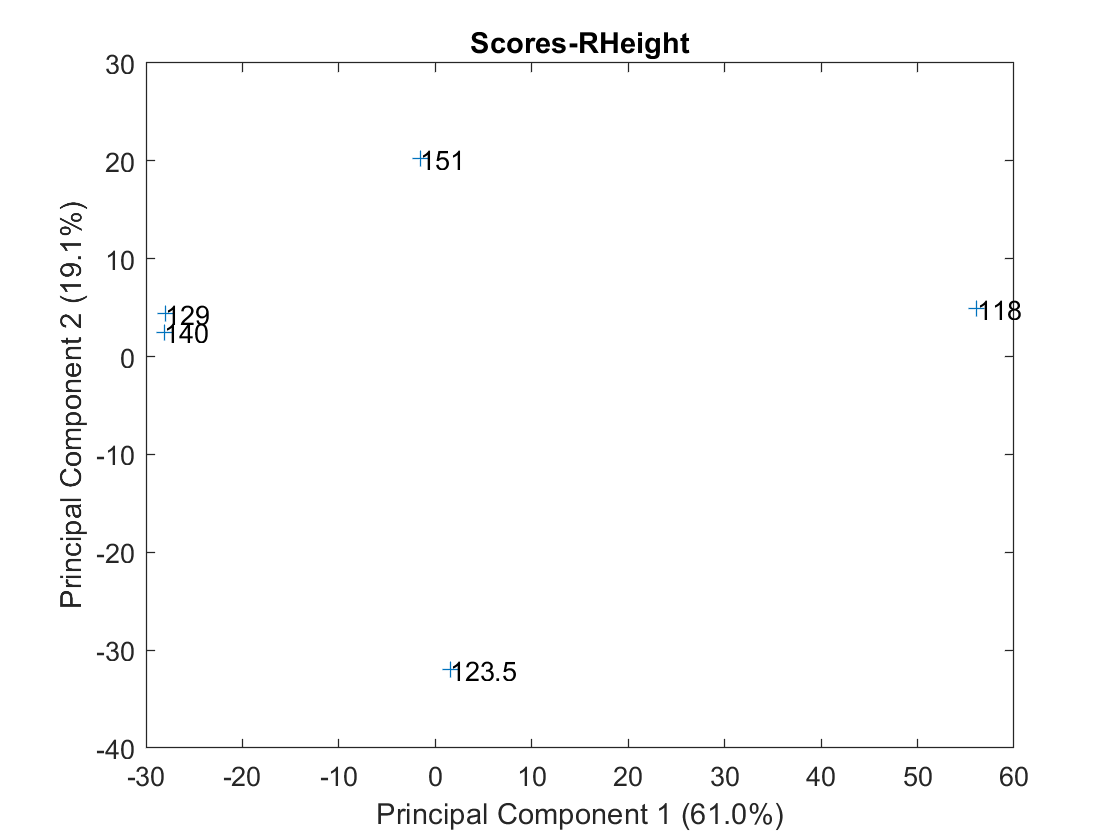
\includegraphics[width=\textwidth]{Figure/DatabehandlingSkalaer/PCAfigures/RHeight-Scores}
\caption{\textit{Score}-plot for PC1 og PC2 i forhold til robottens højde.}
\label{fig:RHeight-Score}
\end{figure}
\noindent
%
Ud fra \textit{Bi}-plottet på \autoref{fig:RHeight-Biplot}, hvorpå \textit{loadings} og \textit{scores} for hver parameter er præsenteret, fremgår det at SQ19 bidrager mest til PC1, SQ1 bidrager mest til PC2 og at SQ5, SQ7, SQ11 og SQ14 forklarer en meget lille del af variansen, hvorfor det ikke giver mening at kommentere på hvordan de indbyrdes ligger, medmindre de indgår i en korrelation med en mere betydende parameter. 
%
\begin{figure}[H]
\centering
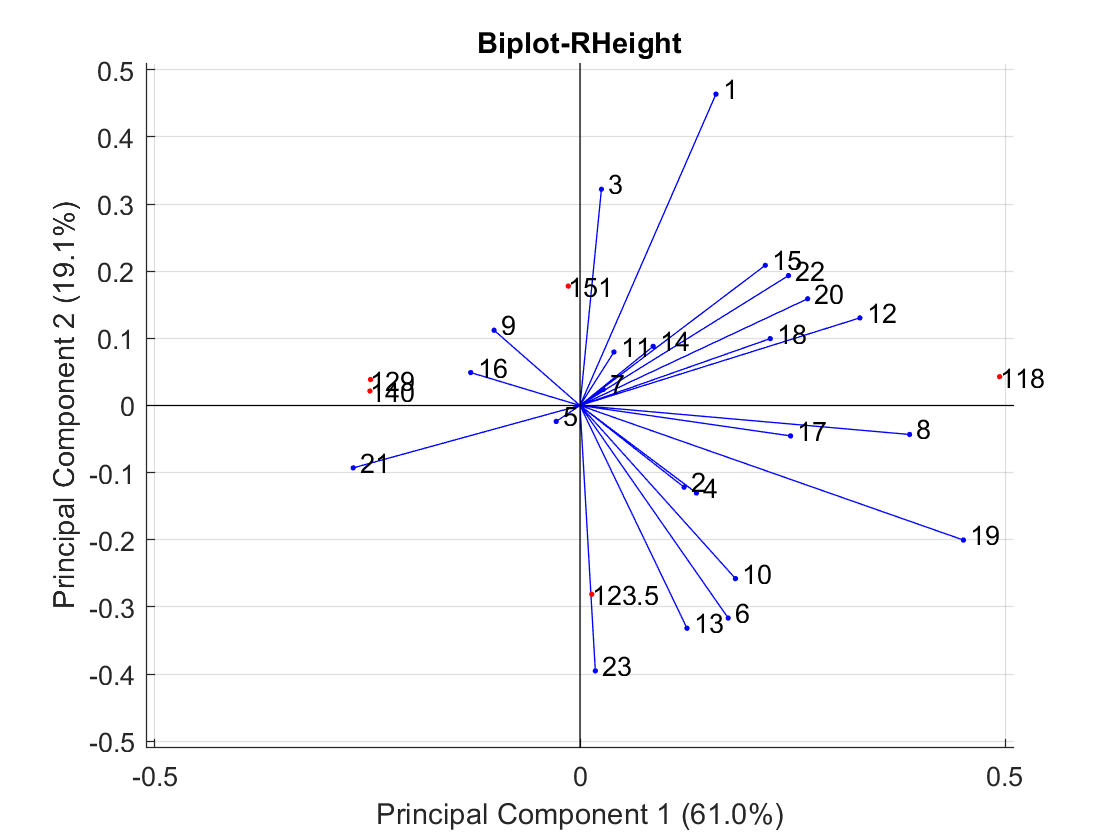
\includegraphics[width=\textwidth]{Figure/DatabehandlingSkalaer/PCAfigures/RHeight-Biplot.png}
\caption{\textit{Bi}-plot med både \textit{loadings} (angivet med blå) og \textit{scores} (angivet med rød) fremgår i forhold til robottens højde.}
\label{fig:RHeight-Biplot}
\end{figure}
\noindent
%
Når to eller flere parametre ligger tæt på hinanden, er det et udtryk for, at de er højt korrelerede. Dette gør sig gældende for SQ2 og SQ4, som henholdvis dækker over hvordan testpersonerne oplevede robotten i forhold til om det er ekstremt afvisende eller ekstremt imødekommende, og hvordan robottens bevægelser blev oplevet i forhold til om bevægelserne er ekstremt rolige eller ekstremt vilde. Lignende er gældende for SQ12 og SQ18, som henholdvist dækker over hvorvidt testpersonerne kan lide, at blive betjent af robotten og om de synes, at robotten er spændende. SQ14 og SQ15 tyder også på at korrelere, da de nærmest ligger oven på hinanden, de to parametre vedrører henholdvist hvor personlig robottens hjælp opleves og hvor overrasket testpersonen blev over robottens henvendelse. Lignende er gældende for SQ8 og SQ17, som også ligger relativt tæt. De to parametre vedrører henholdvist hvorhvidt testpersonerne føler, at robotten kan hjælpe og hvor elegant robotten er. 

Derudover forekommer det at SQ21 er negativt korrelerede med både SQ12 og SQ18, hvor SQ21 vedrører hvor anmassende robotten opleves. SQ9 er negativt korreleret med både SQ2 og SQ4, hvor SQ9 vedrører hvorvidt robotten stod i vejen. Der forekommer også negativ korrelation mellem SQ16, som vedrører hvor irriterende robotten er, og SQ19, som vedrører hvor sød robotten er. Ydermere forekommer der en negativ korrelation mellem SQ3, som vedrører hvor nemt det var at bruge robotten, og SQ23, som vedrører hvor menneskelig robotten oplevels.\blankline
%
I henhold til robottens højde, så ligger 118 cm i modsatte ende af PC1 i forhold til både 129 cm og 140 cm, som nærmest ligger oveni hinanden. Baseret på \autoref{fig:RHeight-Biplot} tyder det derfor på, at højderne 129 cm og 140 cm primært er domineret af SQ21, som vedrører hvor anmassende robotten opleves, og delvist af SQ16, som vedrører hvor irriterende robotten opleves, og SQ9, som vedrører hvorvidt robotten stod i vejen. For højde 118 cm tyder det derimod på, at den højde er domineret af SQ8, som vedrører hvorvidt testpersonen føler, at robotten kan hjælpe en, og delvist af SQ19, som vedrører hvor sød robotten opleves, og SQ12, som vedrører hvor godt testpersonen kan lide at blive betjent af robotten. 

Lignede gør sig gældende for PC2, hvor højderne 123.5 cm og 151 cm adskiller sig. Baseret på \autoref{fig:RHeight-Biplot} fremgår det, at SQ23, som vedrører hvor menneskelig robotten opleves, primært dominerer denne højde. Dertil domineres højden også af SQ13, som vedrører hvorvidt testpersonen regnede med at robotten fulgte dem hen til det sted de havde valgt. Højden på 151 cm er derimod primært domineret af SQ3, som vedrører hvor nemt det var at bruge robotten, samt SQ1, som vedrører skærmens reaktion. \blankline
%
Hver \textit{loading} angiver hvor meget variation hver parameter bidrager med i forhold til den specifikke PC. I \autoref{tab:LoadingsHoejde} fremgår samtlige \textit{loadings} for hver parameter til hver PC.  
%
\begin{table}[H]
\centering
\begin{tabular}{c|c|c|c|c}
    & PC1 (61\%)      & PC2 (19.1\%)    & PC3 (14\%)      & PC4 (5.9\%)     \\ \hline
SQ1  & 0.1598          & \textbf{0.4638} & -0.2199         & -0.0165         \\ \hline
SQ2  & 0.1223          & -0.1217         & 0.0152          & -0.2757         \\ \hline
SQ3  & 0.0252          & 0.3221          & -0.0228         & 0.4574          \\ \hline
SQ4  & 0.1369          & -0.1303         & 0.1984          & 0.0372          \\ \hline
SQ5  & -0.028          & -0.0237         & -0.0339         & -0.1285         \\ \hline
SQ6  & 0.1742          & -0.3167         & \textbf{0.5274} & 0.0873          \\ \hline
SQ7  & 0.0273          & 0.0239          & -0.0078         & -0.0035         \\ \hline
SQ8  & 0.3875          & -0.0432         & -0.2174         & -0.3275         \\ \hline
SQ9  & -0.1010         & 0.1121          & -0.0485         & -0.1130          \\ \hline
SQ10 & 0.1828          & -0.2579         & -0.4600         & 0.0328          \\ \hline
SQ11 & 0.0399          & 0.0796          & 0.1256          & 0.1631          \\ \hline
SQ12 & 0.3290          & 0.1305          & -0.2765         & -0.0732         \\ \hline
SQ13 & 0.1258          & -0.3318         & -0.2525         & \textbf{0.5940} \\ \hline
SQ14 & 0.0860          & 0.0881          & 0.0360          & 0.1441          \\ \hline
SQ15 & 0.2178          & 0.2088          & 0.0282          & -0.1953         \\ \hline
SQ16 & -0.1285         & 0.0490          & 0.0040          & 0.0326          \\ \hline
SQ17 & 0.2475          & -0.0453         & 0.0422          & 0.1889          \\ \hline
SQ18 & 0.2236          & 0.0996          & -0.0310         & 0.1844          \\ \hline
SQ19 & \textbf{0.4507} & -0.2004         & 0.1778          & -0.0131         \\ \hline
SQ20 & 0.2676          & 0.1590          & 0.3334          & -0.0940         \\ \hline
SQ21 & -0.2666         & -0.0929         & 0.0707          & -0.1057         \\ \hline
SQ22 & 0.2451          & 0.1935          & 0.1474          & 0.0239          \\ \hline
SQ23 & 0.0180           & -0.3953        & -0.2013         & -0.1809        
\end{tabular}
\caption{Oversigt over \textit{loadings} til de fire PCs, for hver PC fremhæves den mest betydende parameter. \textit{SQ} angiver skala spørgsmålet.}
\label{tab:LoadingsHoejde}
\end{table}
\noindent
%
Tages der derimod udgangspunkt i et tredimensionelt \textit{Bi}-plot, jævnfør \autoref{fig:RHeight-3D}, fremgår det, at de to højder: 129 cm og 140 cm adskiller sig en del i den tredje dimension. Derudover tyder det på, at SQ6, som vedrører testpersonernes oplevelse af robottens hastighed, samt SQ10, som vedrører hvor tryg testpersonen følte sig ved robotten, er de to parametre, som har størst indflydelse på PC3. 

Derudover elimineres nogen af de førnævnte korrelationer mellem parametrene, når de præsenteres i det tredimensionelle plot, gengivet på \autoref{fig:RHeight-3D}, eller vedlagt i \fullref{ElektroniskBilag3D}. Dette gælder blandt andet SQ2 og SQ4, som ikke længere ligger oven på hinanden, jævnfør ingen korrelation, samt SQ3 og SQ23, der ikke længere er negativt korrelerede. Derudover forefindes det at SQ10 og SQ13 har en svag korrelation.   
%OVERVEJ ET ANDET BILLEDE AF 3D figuren.
\begin{figure}[H]
\centering
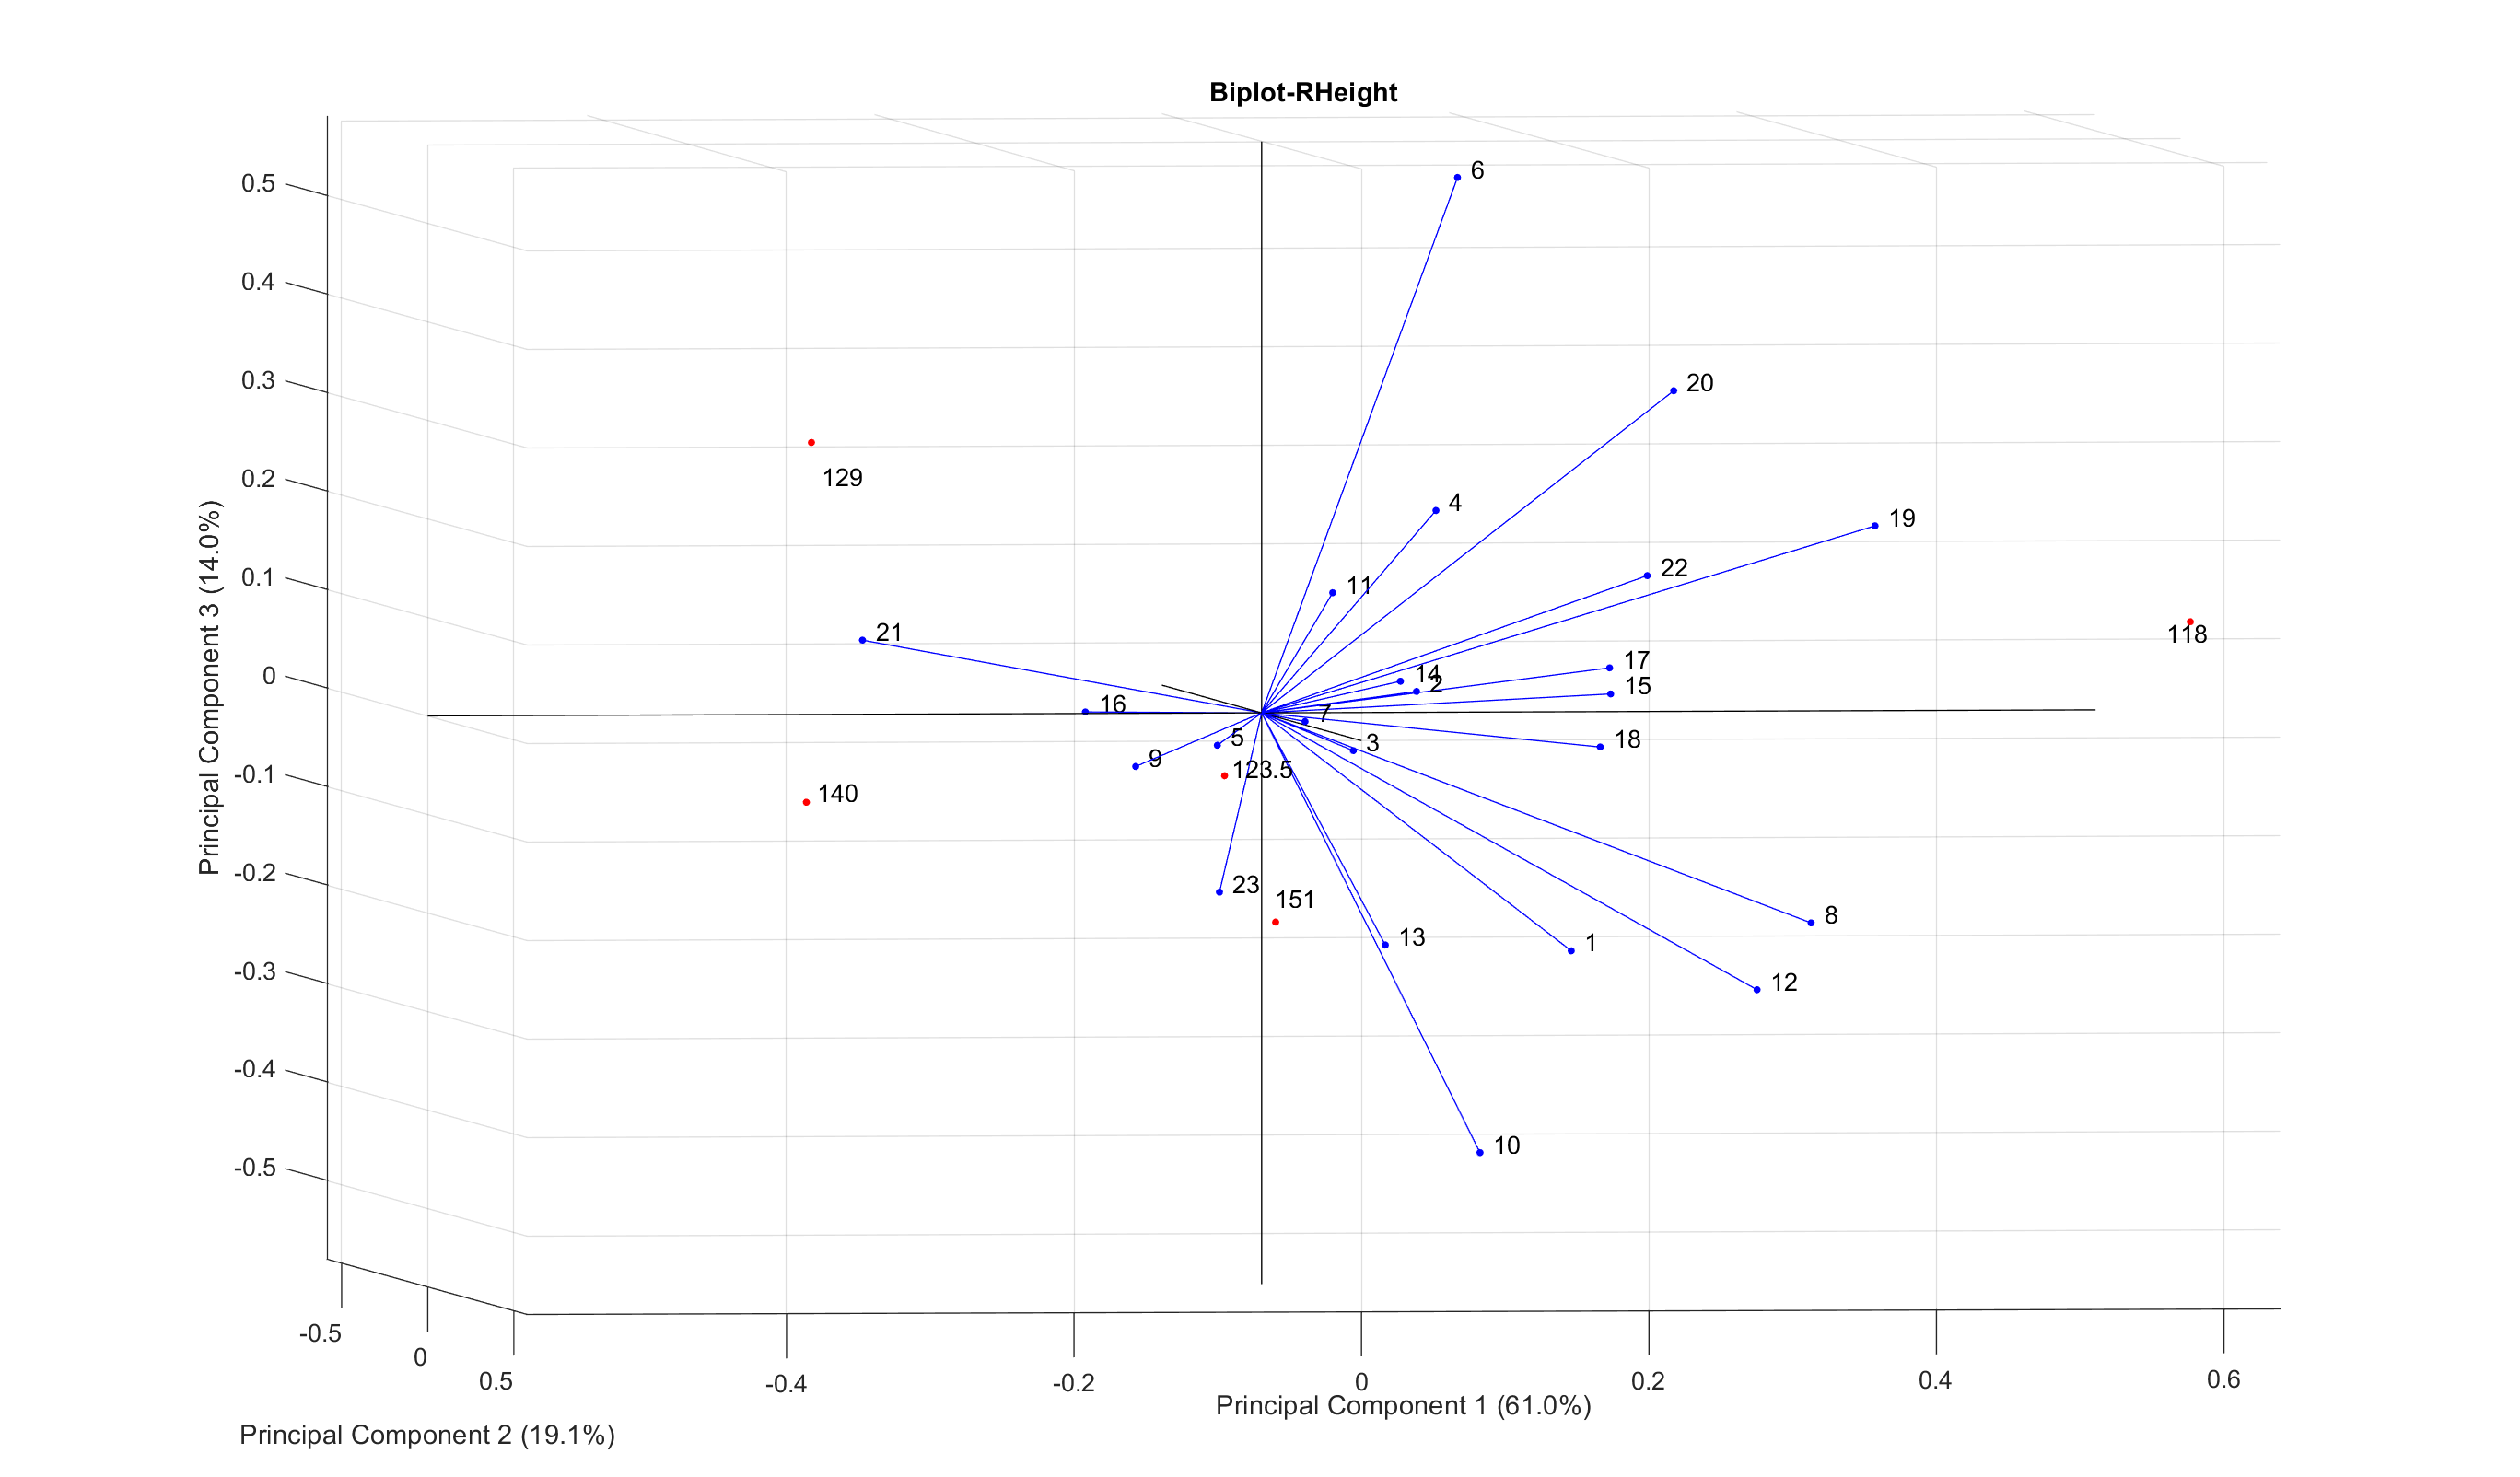
\includegraphics[width=\textwidth]{Figure/DatabehandlingSkalaer/PCAfigures/RHeight-3D.png}
\caption{3D \textit{Bi}-plot med både \textit{loadings} (angivet med blå) og \textit{scores} (angivet med rød) fremgår i forhold til robottens højde.}
\label{fig:RHeight-3D}
\end{figure}
%

\subsection{Tendenser i forhold til robottens højde}
\label{DatabehandlingRHeightTendenser}
%
For at få et indtryk af hvilken indflydelse de fem forskellige højder, fra 118 cm til 151 cm, har på testpersonernes evaluering af interaktionen med robotten, vil der i det følgende afsnit undersøges hvordan højden påvirker parametrene. Undersøgelsen er foretaget på samtlige skalaer, men det vil kun være de skalaer, hvor der er en klar tendens til, at højden påvirker den pågældende parameter, der vil blive præsenteret. Dette vurderes efter, at det højste og laveste punkt på tendenslinjen, den orange stiplede linje, minimum skal variere omkring 10 \% i forhold til y-aksen, som afspejler testpersonernes respons på den specifikke skala. Alle procentsatser er aflæst og ikke udregnet. Testpersonerne er angives ikke kronologisk på x-aksen, da data er sorteret efter laveste og højeste vurdering. Det skal dog understreges, at tendenslinjerne kun er vejledende, da de er manipulerbare i forhold til hvordan datapunkterne struktureres, hvorfor tendenslinjerne skal sammenholdes med kurver de repræsenterer. 

Den første skala hvorpå tendenslinjen ændrer sig med minimum 10 \% er ved SQ4, som vedrører hvordan testpersonen oplevede robottens bevægelse; fra ekstremt rolige (0 \%) til ekstremt vilde (100 \%), hvor variationen aflæses til omkring 21 \%, hvilket fremgår af \autoref{fig:TendensHeightSQ4}. Baseret på dette virker det som om, at der er en tendens til, at desto lavere robotten er, desto vildere opleves dens bevægelser, hvorimod bevægelserne opleves mere rolige desto højere robotten er. 
%
\begin{figure}[H]
\centering
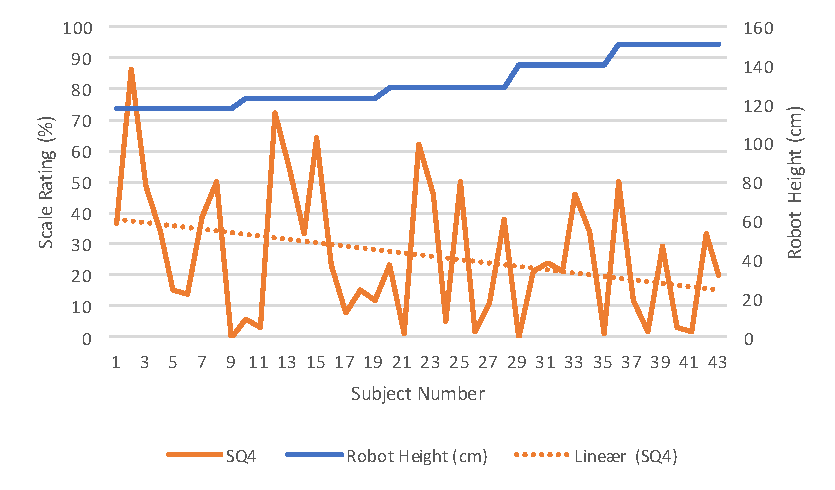
\includegraphics[width=\textwidth]{Figure/DatabehandlingSkalaer/TendensHeight/HeightSQ4}
\caption{Sammenhæng mellem robottens fem højder (cm) og hvad testpersonerne angiver (\%) på skalaen til SQ4: \textit{Hvordan oplevede du robottens bevægelser?}. Denne graf bygger på samtlige 43 besvarelser.}
\label{fig:TendensHeightSQ4}
\end{figure}
\noindent
%
Ud fra \autoref{fig:TendensHeightSQ6} tyder det på, at der er en klar tendens til, at hvis robotten er på sit laveste (118 cm), så opleves robotten som værende omkring 40 \% hurtigere end når robotten er på sit højeste (151 cm).
%
\begin{figure}[H]
\centering
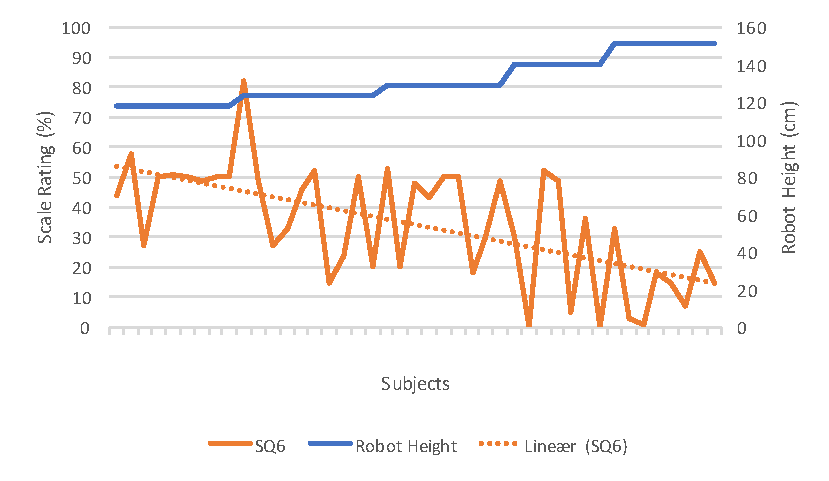
\includegraphics[width=\textwidth]{Figure/DatabehandlingSkalaer/TendensHeight/HeightSQ6}
\caption{Sammenhæng mellem robottens fem højder (cm) og hvad testpersonerne angiver (\%) på skalaen til SQ6: \textit{Jeg synes, at robottens hastighed er...} Denne graf bygger på samtlige 43 besvarelser}
\label{fig:TendensHeightSQ6}
\end{figure}
\noindent
% LIGE PÅ GRÆNSEN
Baseret på \autoref{fig:TendensHeightSQ13} tyder det på, at når robotten er på sit laveste (118 cm), så stoler testpersonerne omkring 18 \% mere på, at robotten følger dem hen til det sted de har valgt, end når robotten er på sit højeste (151 cm). 
%
\begin{figure}[H]
\centering
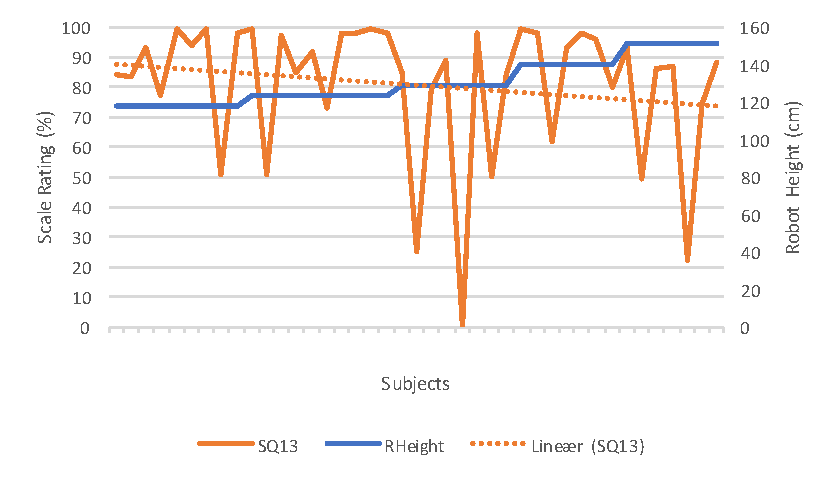
\includegraphics[width=\textwidth]{Figure/DatabehandlingSkalaer/TendensHeight/HeightSQ13}
\caption{Sammenhæng mellem robottens fem højder (cm) og hvad testpersonerne angiver (\%) på skalaen til SQ13: \textit{Jeg regnede med, at robotten fulgte mig hen til det sted jeg valgte}. Denne graf bygger på 41 besvarelser, da der manglede to.}
\label{fig:TendensHeightSQ13}
\end{figure}
\noindent
% 
Baseret på \autoref{fig:TendensHeightSQ17} tyder det på, at når robotten er på sit laveste (118 cm) så opleves den som værende omkring 27 \% mere elegant end når robotten er på sit højeste (151 cm).
%
\begin{figure}[H]
\centering
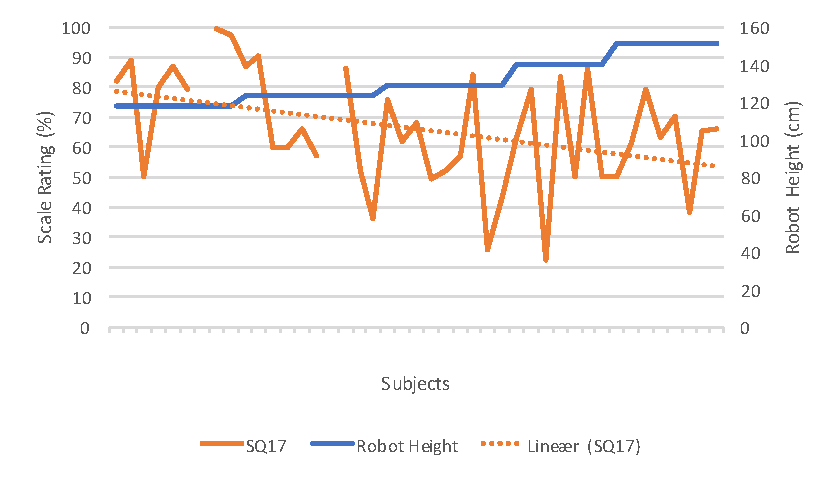
\includegraphics[width=\textwidth]{Figure/DatabehandlingSkalaer/TendensHeight/HeightSQ17}
\caption{Sammenhæng mellem robottens fem højder (cm) og hvad testpersonerne angiver (\%) på skalaen til SQ17: \textit{Hvad synes du om robotten?}, i forhold til \textit{elegant}. Denne graf bygger på 41 besvarelser, da der manglede to.}
\label{fig:TendensHeightSQ17}
\end{figure}
\noindent
%
Baseret på \autoref{fig:TendensHeightSQ19} er der en tendens til, at når robotten er på sit laveste (118 cm) så opleves den omkring 35 \% sødere end når robotten er på sit højeste (151 cm). Dog forekommer der både meget variation mellem de enkelte testpersoner og manglende besvarelser. 
%
\begin{figure}[H]
\centering
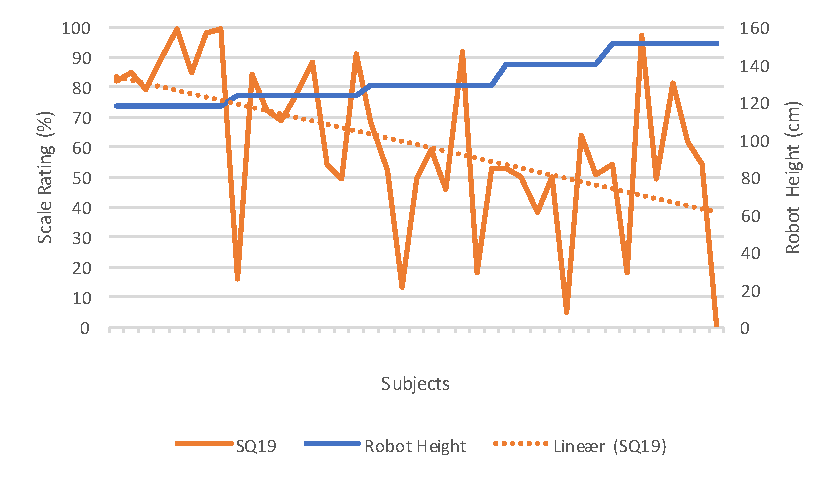
\includegraphics[width=\textwidth]{Figure/DatabehandlingSkalaer/TendensHeight/HeightSQ19}
\caption{Sammenhæng mellem robottens fem højder (cm) og hvad testpersonerne angiver (\%) på skalaen til SQ19: \textit{Hvad synes du om robotten?}, i forhold til \textit{sød}. Denne graf bygger på 41 besvarelser, da der manglede to.}
\label{fig:TendensHeightSQ19}
\end{figure}
\noindent
%
Med forbehold for, at der mangler en del besvarelser til SQ20, omhandlende hvor sej robotten opleves, samt en stor spredning mellem besvarelserne, hvorfor tendenslinjen er fjernet, tyder det på at når robotten er på sit laveste (118 cm) opleves den generelt som værende sejere end på de fire resterende højder, jævnfør \autoref{fig:TendensHeightSQ20}.
%
\begin{figure}[H]
\centering
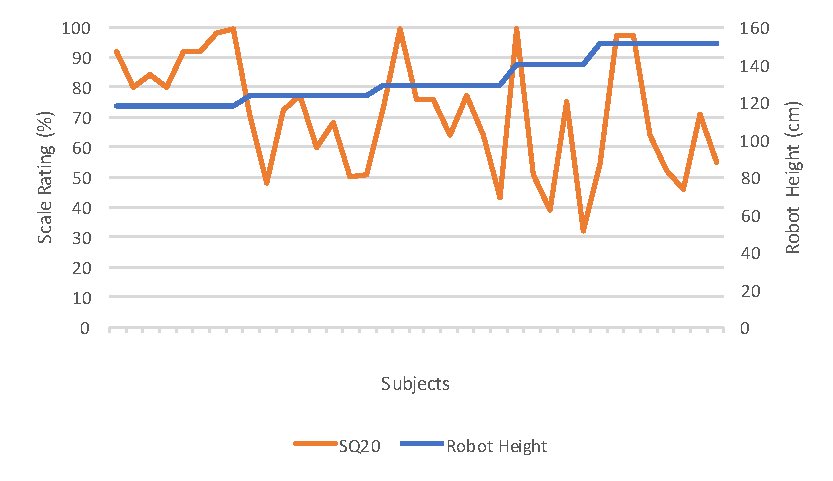
\includegraphics[width=\textwidth]{Figure/DatabehandlingSkalaer/TendensHeight/HeightSQ20}
\caption{Sammenhæng mellem robottens fem højder (cm) og hvad testpersonerne angiver (\%) på skalaen til SQ20: \textit{Hvad synes du ellers om robotten?}, i forhold til \textit{sej}. Denne graf bygger på 37 besvarelser, da der manglede seks.}
\label{fig:TendensHeightSQ20}
\end{figure}
\noindent
%
